 本章では中間発表で記入してもらった評価シートの集計結果とコメントを参考にして今後の改善点を記述する。
 評価シートの評価項目は「発表技術」と「発表内容」の2つと「発表内容」の細部に「ブラックジャックのルール説明の評価」、「検証の評価」の2つ合わせて計4つ用意した。そして、それぞれについて1(非常に悪い)から10(非常に優秀)までの間で評価点を付け、それぞれについてのコメント(評価理由)やアドバイスを記入する欄を用意した。
\bunseki{※葛西隼人}
\section{中間発表}
\subsection{評価点数の集計}
中間発表で記入してもらった評価シートは計42枚だった。シートを記入した人の所属の分布の表\ref{tab:dist} のようになった。

\begin{table}[htb]
  \begin{center}
    \caption{評価人数集計}
    \begin{tabular}{|c|c|c|} \hline 
      所属 & 学年 & 人数  \\ \hline \hline
      教員 &  & 6  \\
      一般 &  & 0 \\
      学生 & 院2年 & 0 \\
     学生 & 院1年 & 0 \\
             & 学部4年 & 1 \\
       & 学部3年 & 34 \\
             & 学部2年 & 1 \\
             & 学部1年 & 0 \\ \hline \hline
      合計 &  & 42 \\ \hline
    \end{tabular}
    \label{tab:dist}
  \end{center}
\end{table}

評価人数の構成としては学部3年が大半を占めていた。その他には教員、学部4年と学部1年から1
人ずつであった。次はそれぞれの評価項目についての平均点を表\ref{tab:point}に記す。

\begin{figure}
\begin{center}
\caption{評価点数集計}
\begin{tabular}{|c|c|c|c|c|c|} \hline
  所属 & 学年 & 発表技術 & 発表内容 & ルール説明 & 検証説明  \\ \hline \hline
  教員 &        & 8 & 7.5 & 7.83 & 7.67 \\
  学生 &        & 6.47 & 7.03 & 7.56 & 6.22 \\
         & 学部2,4年 & 6 & 7 & 5.5 & 7 \\
         & 学部3年 & 6.38 & 7.01 & 7.68 & 6.18 \\ \hline \hline
  全体 &        & 6.69 & 7.1 & 7.6 & 6.43 \\ \hline
\end{tabular}
\label{tab:point}
\end{center}
\end{figure}

全体の平均は「発表技術」については6.69、「発表内容」については7.1、「ルール説明」については7.6、「検証説明」については6.43となった。それぞれの項目について高く評価したのは「教員」だった。
次に、それぞれの結果を図\ref{gizyutu}、図\ref{naiyou}、図\ref{ru-ru}、図\ref{kensyou}に示す。

\begin{figure}[h]
 \begin{tabular}{cc}
  \begin{minipage}[h]{0.45\hsize}
  \centering
 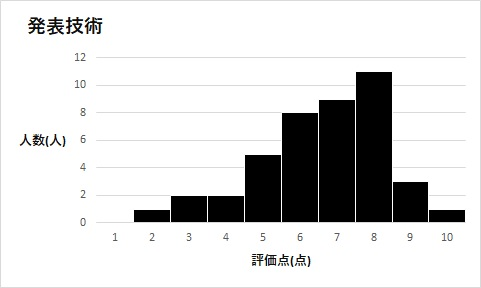
\includegraphics[width=0.7\linewidth]{./figure/gizyutu.jpg}
\caption{発表技術の評価グラフ}
\label{gizyutu}
 \end{minipage} &

\begin{minipage}[h]{0.45\hsize}
  \centering
 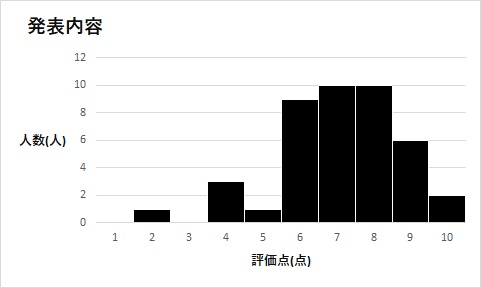
\includegraphics[width=0.7\linewidth]{./figure/naiyou.jpg}
 \caption{発表内容の評価グラフ}
\label{naiyou}
\end{minipage} 
\end{tabular}
\end{figure}

\begin{figure}[h]
 \begin{tabular}{cc}
  \begin{minipage}[h]{0.45\hsize}
  \centering
 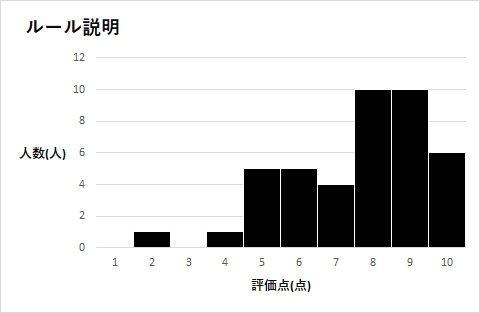
\includegraphics[width=0.7\linewidth]{./figure/ru-ru.jpg}
\caption{ルール説明の評価グラフ}
\label{ru-ru}
 \end{minipage} &

\begin{minipage}[h]{0.45\hsize}
  \centering
 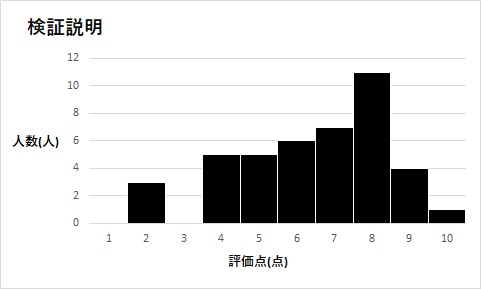
\includegraphics[width=0.7\linewidth]{./figure/kensyou.jpg}
 \caption{検証説明の評価グラフ}
\label{kensyou}
\end{minipage} 
\end{tabular}
\end{figure}
「発表技術」と「発表内容」については評価点が共に7、8点と高い評価点が多かった。ルール説明についても同様に高い評価点が多かった、一方で検証説明については4、5点が多い結果となった。

また、「発表技術」と「発表内容」の評点の相関係数は0.71となった。これは2つの評価項目がかなり関連してると言える数値である。次にコメントについて解析する。
\bunseki{※葛西隼人}

\subsection{コメント解析と改善点}
まず、「発表技術」について、肯定的なコメントと否定的なコメントに分けて並べる。
肯定的なコメント
\begin{itemize}
\item 複雑な内容をうまく説明してくれた
\item スライド内で図を多用されていて分かりやすかった
\end{itemize}

否定的なコメント
\begin{itemize}
\item 前を見て話してもらえないと聞き取りにくい
\item 説明が少し早い
\item プレゼンの内容が構造的でないために、全体に対して今どの部分を話しているのかわかりにくい
\end{itemize}

今回はスライドの分量が多く、どうしても早口になってしまったのでこのような意見が多かった。そしてスライドの完成が遅かったために構成までについて詳しく話し合うことができなかった。また発表の練習時間が取れなかったために技術面で足りない点もいくつかコメントで述べられていた。
次に、「発表内容」についても同様に、コメントを肯定的なコメントと否定的なコメントに分けて並べる。
肯定的なコメント
\begin{itemize}
\item 活動内容が明確でよかった
\item 実験・検証が多く、説得力をもたせている
\item 評価基準や比較対象が明確で理解しやすかった
\end{itemize}

否定的なコメント
\begin{itemize}
\item 用語についてより詳しく説明すべき
\item 聞く人の知識が必要になるのでもう少しわかりやすく
\item 検証結果のみせ方にもう少し工夫があると良かった。(専門的な知識がない人にもわかりやすく)
\end{itemize}

「発表内容」に関しては、ブラックジャックのルール説明はわかりやすいとのコメントが多かった。しかし検証の説明はあまり理解出来ないとのコメントも見受けられた。最後に「発表内容」と「発表技術」の2つのコメント欄から重要なアドバイスがいくつかあったため、これらについても述べていく。 
\begin{itemize}
\item なぜあのような式を利用することで性能が表されているかの説明がもう少し欲しかった
\item 文字数を減らし簡潔な内容の方がいいと思う
\item スライドに色を使って見やすくしたほうが良い
\item 基本的に文字がたくさんのスライドで、太字や下線などもなかったので、どこに注目してよいかわからなかった。後期の発表ではもっとスライドを効果的に見せてほしい
\end{itemize}
これらの意見に関しても、後期の活動に反映することとする。
以上より中間発表の評価コメントは賛否両論であり、とても参考になった。
\bunseki{※葛西隼人}